\documentclass[11pt,DIV=12,a4paper,abstract=true,twoside=semi,openright]
{scrreprt}
\usepackage[T1]{fontenc}
\usepackage[USenglish]{babel}
\usepackage[varqu,varl]{zi4}% inconsolata typewriter
% for lualatex
\usepackage{fontspec}
\setmonofont{Inconsolatazi4}
\usepackage[sfdefault,scaled=.85]{FiraSans}
\usepackage[cmintegrals]{newtxsf}
\usepackage{csquotes}
\usepackage{isabelle,isabellesym}
\usepackage{booktabs}
\usepackage{graphicx}
\usepackage{xspace}
\usepackage{xcolor}
\usepackage{listings}
\usepackage[]{mathtools}
\usepackage{railsetup}
\usepackage[backend=bibtex,style=trad-abbrv]{biblatex}
\addbibresource{root.bib}


\usepackage[pdfpagelabels, pageanchor=false, plainpages=false]{hyperref}
\usepackage{orcidlink}

%\renewcommand\familydefault{\sfdefault}
\colorlet{sectioncolor}{blue!60!black}
\addtokomafont{chapterentrypagenumber}{\color{sectioncolor}}
\addtokomafont{chapterentry}{\color{sectioncolor}}
\addtokomafont{title}{\color{sectioncolor}\bfseries}
\addtokomafont{chapter}{\color{sectioncolor}\bfseries}
\addtokomafont{section}{\color{sectioncolor}}
\addtokomafont{subsection}{\color{sectioncolor}}
\addtokomafont{subsubsection}{\color{sectioncolor}}
\addtokomafont{paragraph}{\color{sectioncolor}}
\addtokomafont{subparagraph}{\color{sectioncolor}}

\renewcommand{\isastyletext}{\normalsize\normalfont\sffamily}
\renewcommand{\isastyletxt}{\normalfont\sffamily}
\renewcommand{\isastylecmt}{\normalfont\sffamily}

\isabellestyle{literal}
\isabellestyle{tt}

\setcounter{tocdepth}{3}
\newcommand{\ie}{i.\,e.\xspace}
\newcommand{\eg}{e.\,g.\xspace}
\newcommand{\thy}{\isabellecontext}
\renewcommand{\isamarkupsection}[1]{%
  \begingroup% 
  \def\isacharunderscore{\textunderscore}%
  \section{#1 (\thy)}%
  \endgroup% 
}
\let\oldisakeyword\isakeyword
\renewcommand{\isakeyword}[1]{\oldisakeyword{\color{black!70!white}#1}}
\renewcommand{\isacommand}[1]{\isakeyword{\color{sectioncolor}#1}}

\title{Nano JSON}
\subtitle{Working with JSON formatted data in Isabelle/HOL and Isabelle/ML} 
\author{Achim~D.~Brucker\textsuperscript{\orcidlink{0000-0002-6355-1200}}}%
\publishers{
  Department of Computer Science, University of Exeter, Exeter, UK\texorpdfstring{\\}{, }
  \texttt{a.brucker@exeter.ac.uk}
}

\begin{document}
  \maketitle
  \begin{abstract}
    \begin{quote}
      JSON (JavaScript Object Notation) is a common format for exchanging data,
      based on a collection of key/value-pairs (the JSON objects) and lists. Its
      syntax is inspired by JavaScript with the aim of being easy to read and
      write for humans and easy to parse and generate for machines. 
  
      Despite its origin in the JavaScript world, JSON is language-independent
      and many programming languages support working with JSON-encoded data.
      This makes JSON an interesting format for exchanging data with
      Isabelle/HOL.
 
      This AFP entry provides a JSON-like import-expert format for both
      Isabelle/ML and Isabelle/HOL. On the one hand, this AFP entry provides
      means for Isabelle/HOL users to work with JSON encoded data without the
      need using Isabelle/ML. On the other and, the provided Isabelle/ML
      interfaces allow additional extensions or integration into Isabelle
      extensions written in Isabelle/ML. While format is not fully JSON
      compliant (e.g., due to limitations in the range of supported Unicode
      characters), it works in most situations: the provided implementation in
      Isabelle/ML and its representation in Isabelle/HOL have been used
      successfully in several projects for exchanging data sets of several
      hundredths of megabyte between Isabelle and external tools.

      \bigskip
      \noindent\textbf{Keywords:} JSON, JavaScript Object Notation, data
        exchange, data import, data export 
    \end{quote}
  \end{abstract}
\tableofcontents


\chapter{Introduction}
JSON (JavaScript Object Notation)~\cite{ecma:json:2017,ietf:rfc8259-json:2017}
is a widely-used format for exchanging data, having replaced
XML~\cite{bray.ea:extensible:2008} in many areas. The structure of JSON is based
on:
\begin{itemize}
\item A collection of key-value (name-value) pairs, also called JSON object. In
  programming languages, this corresponds, e.g., to data structures such as
  objects, records, structs, or hash tables. 
\item A finite list of values. In programming languages, this corresponds, e.g.,
  to lists, sequences, or arrays. 
\end{itemize}
The syntax of  is inspired by JavaScript with the aim of being easy to read and
write for humans (that are comfortable with curly-bracket programming languages)
and easy to parse and generate for machines. 

Despite its origin in the JavaScript world, JSON is language-independent and
many programming languages support working with JSON-encoded data. This makes
JSON an interesting format for exchanging data with Isabelle/HOL.
 
This AFP entry provides a JSON-like import-expert format for both Isabelle/ML
and Isabelle/HOL. While this entry provides a simple formal model of JSON,
formalizing an object-based data structure is not the aim of this AFP entry (for
this, see,
e.g.,~\cite{brucker.ea:extensible:2008-b,brucker.ea:afp-core-dom:2018}). The aim
of this AFP entry is to provide means to work with JSON-encoded data in
Isabelle, similar to the AFP entry ``XML''~\cite{sternagel.ea:xml:2014} provides
means to work with XML documents in Isabelle. 

In more detail, this AFP entry provides two different ways for importing and
exporting JSON-encoded data in Isabelle:
\begin{labeling}{\textbf{Isabelle/HOL:}}
\item[\textbf{Isabelle/HOL:}] This AFP entry provides means for Isabelle/HOL
      users to work with JSON encoded data: it provides a HOL data type
      modelling the JSON format and new top-level
      Isar~\cite{wenzel:isabelleisar:2002} commands to import and export JSON
      encoded files. Moreover, a new top-level Isar command is provided to parse
      JSON data that is stored ``inline'' within the Isabelle/HOL theory file. 
\item[\textbf{Isabelle/ML:}] This AFP entry also provides interfaces to the
      underlying implementation in Isabelle/ML, allowing to write users to
      write their on extensions that require features not (yet) exposed to the 
      Isabelle/HOL level. For example, data type packages for specific variants of JSON
      that, e.g., should directly map to specific HOL data types or that need
      further encoding or conversions during export or import. 
\end{labeling}

While the supported JSON-variant is not fully JSON compliant (e.g., due to
limitations in the range of supported Unicode characters), it works in most
situations: the provided implementation in Isabelle/ML and its representation in
Isabelle/HOL have been used successfully in several projects for exchanging data
sets of several hundredths of megabyte between Isabelle and external tools.


In summary, Nano JSON should enable you to work with JSON encoded data in
Isabelle/HOL without the need of implementing parsers or serialization in
Isabelle/ML. You should be able to implement mapping from the Nano JSON HOL data
types to your own data types on the level of Isabelle/HOL (i.e., as executable
HOL functions). Nevertheless, the provided ML routine that converts between the
ML representation and the HOL representation of Nano JSON can also serve as a
starting point for converting the ML representation to your own,
domain-specific, HOL encoding. 


\begin{figure}
  \centering
  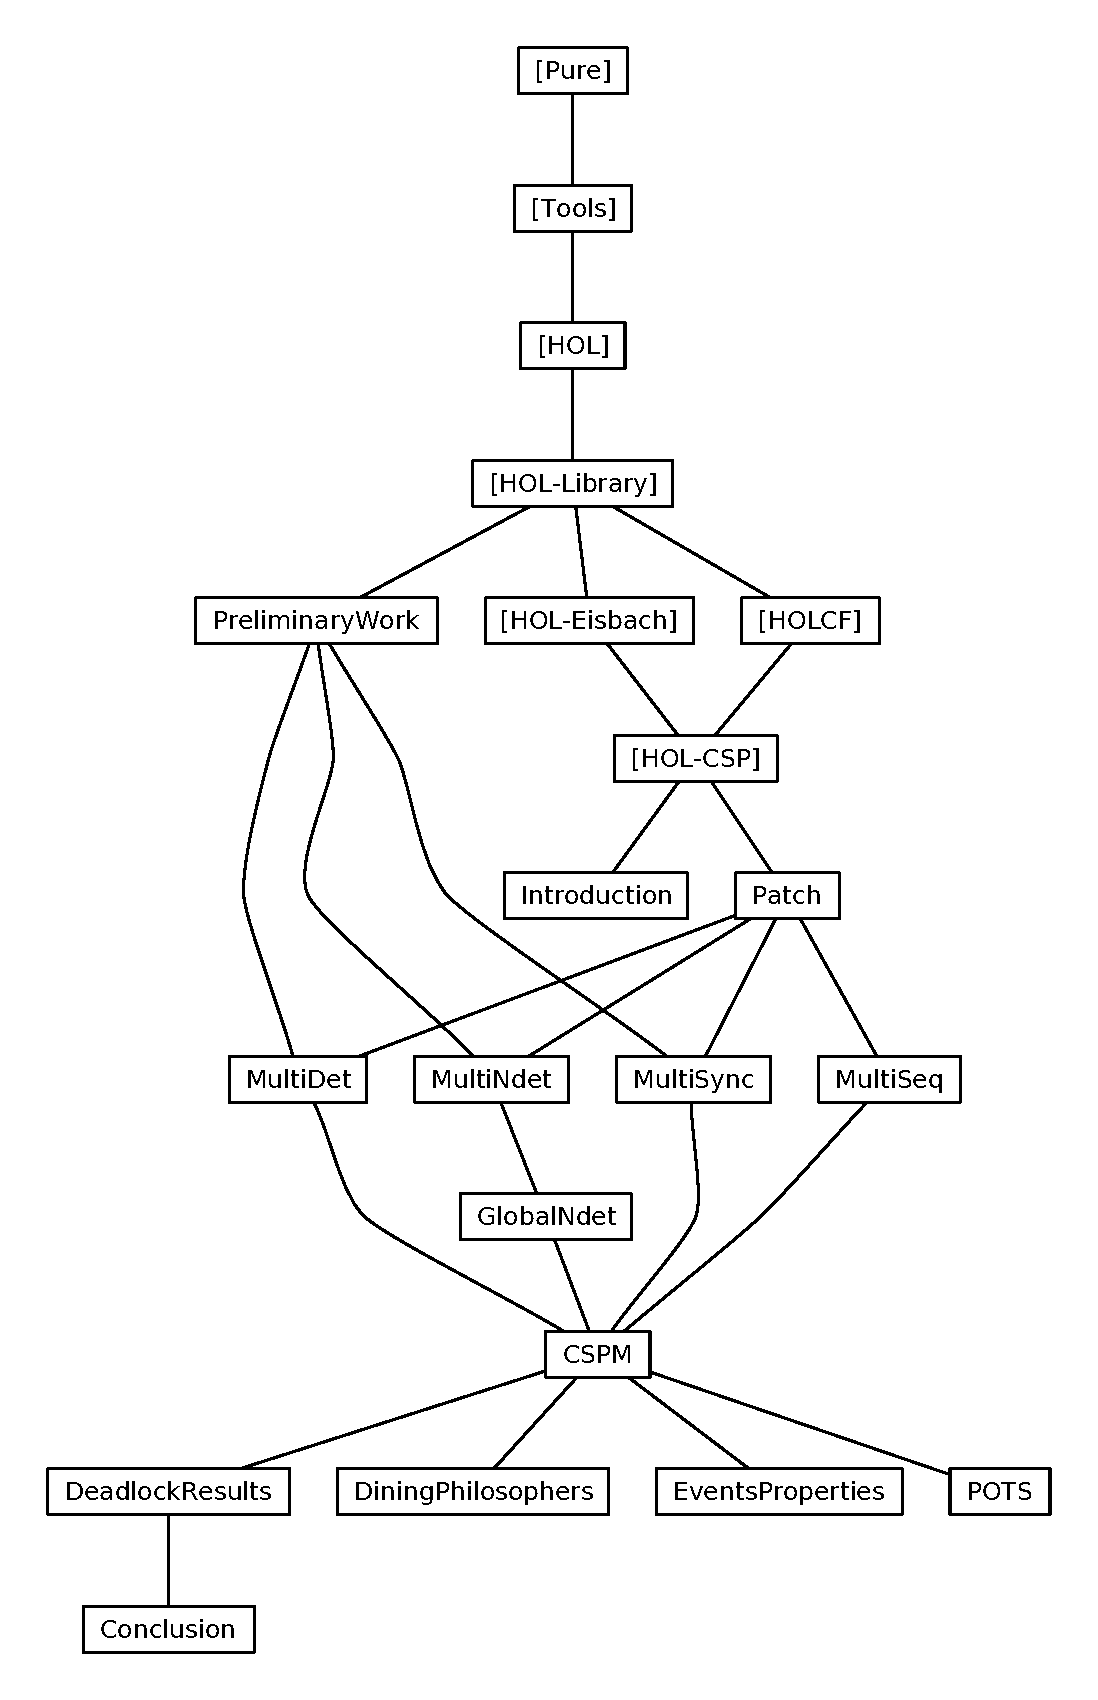
\includegraphics[height=.45\textheight, width=\textwidth, keepaspectratio]{session_graph}
  \caption{The Dependency Graph of the Isabelle Theories.\label{fig:session-graph}}
\end{figure}
The rest of this document is automatically generated from the formalization in Isabelle/HOL, i.e., 
all content is checked by Isabelle.  Overall, the structure of this document follows the theory 
dependencies (see \autoref{fig:session-graph}). If you want  to understand the implementation of 
Nano JSON or want to use its API on the level of Isabelle/ML, you should consult \autoref{ch:implementation}.
If you are interested in using Nano JSON on the level of Isabelle/HOL or want to explore examples, 
please consult \autoref{ch:user-guide}.

\chapter{Implementation}\label{ch:implementation}
\input{Nano_JSON.tex}
\input{Nano_JSON_Query.tex}
\input{Nano_JSON_Main.tex}

\chapter{User's Guide and Examples}\label{ch:user-guide}
\input{Nano_JSON_Manual.tex}
\input{Example.tex}
\input{Example_Real.tex}

%\chapter{Generated Sessions}
% generated text of all theories
%\input{session}

\printbibliography

\end{document}

%%% Local Variables:
%%% mode: latex
%%% TeX-master: t
%%% End:
